\chapter{Simple Beginnings}\label{basics}

We begin by introducing the basic elements of R.
You'll use these elements less often than you might expect,
but they are the building blocks for the higher-level tools introduced in Chapter~\ref{tidyverse},
and concepts like data types, vectors, and loops have direct comparisons in other languages.

Where comparisons might aid understanding,
I'll provide short examples in Python.

\section{Hello World}

We begin with the traditional greeting.
In Python, we would write:

\begin{lstlisting}
print("Hello, world!")
\end{lstlisting}
And this would output:
\begin{lstlisting}
Hello, world!
\end{lstlisting}

The equivalent R looks exactly the same,
and produces very similar output when we run it in the RStudio Console (Figure~\ref{fig:console}):

\begin{lstlisting}
print("Hello, world!")
\end{lstlisting}
And we receive the same output:
\begin{lstlisting}
[1] "Hello, world!"
\end{lstlisting}

% GW FIXME: edit the image to circle it in red.

\begin{figure}[h]
  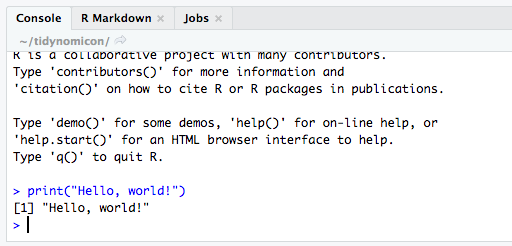
\includegraphics[width=7.11in]{figures/basics/console}
  \caption{RStudio Console}
  \label{fig:console}
\end{figure}

Python prints only what we asked for,
but notice that the R output has a \texttt{[1]}.
You may be mistaken in thinking it's something akin to a line number.
Let's take a closer look by evaluating a couple of expressions without calling \texttt{print}:

\begin{lstlisting}
'This is in single quotes.'
"This is in double quotes."
\end{lstlisting}

This outputs:

\begin{lstlisting}
[1] "This is in single quotes."
[1] "This is in double quotes."
\end{lstlisting}

\texttt{[1]} doesn't appear to be a line number;
it is, in fact, the index of the first element of that line.
When we print vectors with dozens or hundreds of elements,
having the index in the output makes it much easier to locate specific values.

\begin{quote}
\textbf{Single and Double Quotes}

Note that in R we use double quotes to display strings even when we give it a single-quoted string,
in the same way Python using single quotes when we've given it doubles.
\end{quote}

\section{Adding Numbers}

In Python,
we add numbers using \texttt{+} like so:

\begin{lstlisting}
print(1 + 2 + 3)
\end{lstlisting}

\begin{lstlisting}
6
\end{lstlisting}

The equivalent in R is the same but doesn't require the print statement:

\begin{lstlisting}
1 + 2 + 3
\end{lstlisting}

\begin{lstlisting}
[1] 6
\end{lstlisting}

We can check the type of the result using \texttt{type},
which tells us that the result \texttt{6} is an integer:

\begin{lstlisting}
print(type(6))
\end{lstlisting}

\begin{lstlisting}
<class 'int'>
\end{lstlisting}

In R we check the type using:

\begin{lstlisting}
typeof(6)
[1] "double"
\end{lstlisting}

R's type inspection function is \texttt{typeof} rather than \texttt{type},
and it returns the type's name as a string.
That's all fine for finding the type,
but notice that our integer addition has produced a double-precision floating-point result.
Let's try an experiment to explore why:

\begin{lstlisting}
typeof(6)
[1] "double"
\end{lstlisting}

Ah: by default,
R represents numbers as floating-point values,
even if they look like integers when written.
We can force a literal value to be an integer by appending an upper-case \texttt{L},
which stands for ``long integer'':

\begin{lstlisting}
typeof(6L)
[1] "integer"
\end{lstlisting}

(We don't actually need integers very often,
but most other languages have them,
and R might feel left out if they weren't available.)

% LC maybe say why it would be useful to convert to an integer -- are there cirumstanced when an integer is preferable over the default floating point?
% GW not really these days, but they're traditional... Sentences amended above.

Arithmetic on integers does produce integers:

\begin{lstlisting}
typeof(1L + 2L + 3L)
[1] "integer"
\end{lstlisting}

We can also convert a floating-point number to an integer:

\begin{lstlisting}
typeof(as.integer(6))
[1] "integer"
\end{lstlisting}

Notice the dot in \texttt{as.integer}'s name.
If you're coming from Python you might assume there's an object called \texttt{as}
with a \gref{g:method}{method} called \texttt{integer}.
In actuality,
\texttt{.} is (usually) just another character in R used to make names more readable, 
like the underscore \texttt{\_}.

\section{Storing Numbers Together}

The Elder Gods do not bother to learn most of our names
because there are so many of us and we are so ephemeral.
Similarly, we only give a handful of values in our programs their own names; these named values are \emph{variables}.

We lump the rest of the values together into lists, matrices, and more esoteric structures
so that we too, like the Gods, can create, manipulate, and dispose of multitudes with a single imperious command.

The most common such structure in Python is the list.
We create lists using square brackets
and assign a list to a variable using \texttt{=}.
If the variable doesn't already exist, it is created:

\begin{lstlisting}
primes = [3, 5, 7, 11]
print(primes)
\end{lstlisting}

\begin{lstlisting}
[3, 5, 7, 11]
\end{lstlisting}

Since assignment is a \gref{g:statement}{statement}
rather than an \gref{g:expression}{expression},
it has no result,
so Python does not display anything when this command is run. You must explicitly use it after the list is created.

The equivalent to a list  in R is  a \gref{g:vector}{vector}:

\subsection{Creating Vectors}

You build a vector using a function called \texttt{c},
which stands for ``column'':

\begin{lstlisting}
primes <- c(3, 5, 7, 11)
primes
[1]  3  5  7 11
\end{lstlisting}

We enter the name we want to give the list and assign the list using a left-pointing arrow \texttt{\textless{}-}
(though other forms of assignment exist, which we will discuss later).
As in Python,
assignment is a statement rather than an expression,
so we must enter the name of the newly-created variable to get R to display its value.

\subsection{Vector Types}

Vector types in R behave differently to list types in Python.
To explore this let's look at the length of a list, first in Python:

\begin{lstlisting}
print(len(primes))
\end{lstlisting}

\begin{lstlisting}
4
\end{lstlisting}

Let's try the same with the single value 4:

\begin{lstlisting}
print(len(4))
\end{lstlisting}

\begin{lstlisting}
Error in py_call_impl(callable, dots$args, dots$keywords): TypeError: object of type 'int' has no len()

Detailed traceback: 
  File "<string>", line 1, in <module>
\end{lstlisting}

As you may expect, we get an error:
the length of a list is the number of elements it contains,
and since a \gref{g:scalar}{scalar} like the integer 4 doesn't contain elements,
it has no length.

Now we'll print the lengths of our R vector

\begin{lstlisting}
length(primes)
[1] 4
\end{lstlisting}

This is as we expect. And the same with a single value:

\begin{lstlisting}
length(4)
[1] 1
\end{lstlisting}

The value 4 has a length of 1, which may surprise you.
This is because \emph{there are no scalars in R}:
\texttt{4} is not a single lonely integer,
but rather a vector of length one containing the value 4.

Let's have a closer look at the type of our \lstinline{primes} vector:

\begin{lstlisting}
typeof(primes)
[1] "double"
\end{lstlisting}

The type of the vector is the type of the elements it contains.

The last thing to note is that when we display a vector,
the \texttt{[1]} that R prints is the index of its first value, as mentioned earlier.
We can prove this by creating and displaying a longer vector:

\begin{lstlisting}
c(1, 2, 3, 4, 5, 6, 7, 8, 9, 10, 1, 2, 3, 4, 5, 6, 7, 8, 9, 10,
  1, 2, 3, 4, 5, 6, 7, 8, 9, 10, 1, 2, 3, 4, 5, 6, 7, 8, 9, 10)
 [1]  1  2  3  4  5  6  7  8  9 10  1  2  3  4  5  6  7  8  9 10  1  2  3
[24]  4  5  6  7  8  9 10  1  2  3  4  5  6  7  8  9 10
\end{lstlisting}

In order to help us find our way in our data,
R automatically breaks long lines
and displays the starting index of each line.
These indices also show us that R counts from 1 as humans do,
rather than from zero.
(There are a great many myths about why programming languages do the latter.
\href{http://exple.tive.org/blarg/2013/10/22/citation-needed/}{The truth is stranger than any fiction could be.})

\subsection{Indexing with Vectors}

Python's rules for indexing are simple once you understand them
(a statement which is also true of quantum mechanics and necromancy).

To avoid confusing indices with values,
let's create a list of color names and index that, first in Python:

\begin{lstlisting}
colors = ["eburnean", "glaucous", "wenge"]
print(colors[0])
\end{lstlisting}

If we want to access the first element in the list, we simply give the index 0; if we want the second, we give the index 1, and so on:

\begin{lstlisting}
eburnean
\end{lstlisting}


\begin{lstlisting}
print(colors[2])
\end{lstlisting}

\begin{lstlisting}
wenge
\end{lstlisting}

When we try to retrieve an index outside of the existing range, we get an error:

\begin{lstlisting}
colors[3]
\end{lstlisting}

\begin{lstlisting}
Error in py_call_impl(callable, dots$args, dots$keywords): IndexError: list index out of range

Detailed traceback: 
  File "<string>", line 1, in <module>
\end{lstlisting}

And using a negative index begins the count at the end of the list:

\begin{lstlisting}
***print(colors[-1])***
wenge
\end{lstlisting}

Let's index the equivalent vector in R with the indices 1 to 3:

\begin{lstlisting}
colors <- c("eburnean", "glaucous", "wenge")
colors[1]
\end{lstlisting}

\begin{lstlisting}
[1] "eburnean"
\end{lstlisting}

\begin{lstlisting}
colors[3]
\end{lstlisting}

\begin{lstlisting}
[1] "wenge"
\end{lstlisting}

And here's what happens when you go out of bounds:

\begin{lstlisting}
colors[4]
\end{lstlisting}

\begin{lstlisting}
[1] NA
\end{lstlisting}

R handles gaps in data using the special value \gref{g:NA}{\texttt{NA}} (short for ``not available''),
and returns this value when we ask for a nonexistent element of a vector.
But indexing in R does more than this---much more, as we'll see.

In R,
we use a negative index to indicate a value that we don't want, and so retrieve all elements except the one given at the negative index:

\begin{lstlisting}
colors[-1]
\end{lstlisting}

\begin{lstlisting}
[1] "glaucous" "wenge"   
\end{lstlisting}

Now the astute reader will be thinking: if every value in R is a vector,
then when we use 1 or -1 as an index,
we're actually using a vector to index another vector.
What happens if we use a vector with more than one value to index?
Let's create a vector with \texttt{c(...)} and use that as an index.

\begin{lstlisting}
colors[c(3, 1, 2)]
\end{lstlisting}

\begin{lstlisting}
[1] "wenge"    "eburnean" "glaucous"
\end{lstlisting}

That works to retrieve multiple elements, and also allows us to request repeat elements:

\begin{lstlisting}
colors[c(1, 1, 1)]
\end{lstlisting}

\begin{lstlisting}
[1] "eburnean" "eburnean" "eburnean"
\end{lstlisting}

This is known as \gref{g:pull-indexing}{pull indexing}:
the value at location \emph{i} in the index vector specifies which element of the source vector
to pull into that location in the result vector (Figure~\ref{fig:pull-indexing}).

\begin{figure}[h]
  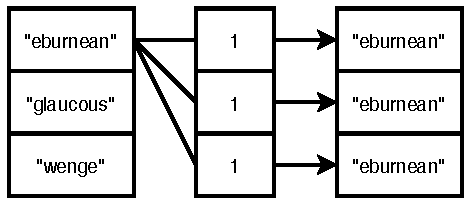
\includegraphics{figures/basics/pull-indexing.pdf}
  \caption{Pull Indexing}
  \label{fig:pull-indexing}
\end{figure}

R requires you to use a vector of indices
and not just use the indices on their own. If you tried to use regular indices, you'd get an error:

\begin{lstlisting}
colors[1, 2]
\end{lstlisting}

\begin{lstlisting}
Error in colors[1, 2]: incorrect number of dimensions
\end{lstlisting}

That didn't work because R interprets \texttt{[i,\ j]} as being
row and column indices for a two-dimensional matrix,
and our vector has only one dimension.

We can also use vectors of negative indices.
Since one negative index selects out one value,
multiple negative indices select out multiple values:

\begin{lstlisting}
colors[c(-1, -2)]
\end{lstlisting}

\begin{lstlisting}
[1] "wenge"
\end{lstlisting}

However,
R won't simultaneously select elements in (with positive indices) and out (with negative ones),
since it's all too easy to wind up with an ambiguous statement
that simultaneously does and doesn't ask for a particular element:

\begin{lstlisting}
colors[c(1, -1)]
\end{lstlisting}

\begin{lstlisting}
Error in colors[c(1, -1)]: only 0's may be mixed with negative subscripts
\end{lstlisting}

We get an error message as expected. However, that error message is suggestive:
Let's see what happens if we use 0 as an index:

\begin{lstlisting}
colors[0]
\end{lstlisting}

\begin{lstlisting}
character(0)
\end{lstlisting}

That's{\ldots}interesting.
The result doesn't include an index in square brackets,
and looks like a function call.
To try to understand what it means,
we'll call the function \texttt{character} ourselves
with a positive argument:

\begin{lstlisting}
character(3)
\end{lstlisting}

\begin{lstlisting}
[1] "" "" ""
\end{lstlisting}

This shows us that 
\texttt{character(N)} constructs a vector of empty strings of the specified length.
The expression \texttt{character(0)} presumably therefore means
``an \gref{g:empty-vector}{empty vector} of type character''.
From this,
we conclude that the index 0 doesn't correspond to any elements,
so R gives us back something of the right type but with no content.
To check if this assumption is right,
let's try indexing with 0 and 1 together:

\begin{lstlisting}
colors[c(0, 1)]
\end{lstlisting}

\begin{lstlisting}
[1] "eburnean"
\end{lstlisting}

This shows that when 0 is mixed with either positive or negative indices,
the 0 is ignored and we get the value at \lstinline{1}.
This outcome can  lead to some puzzling bugs,
as we wind up with fewer values than we had indices.

Finally,
let's look at what happens you mix in-bounds and out-of-bounds indices are mixed:

\begin{lstlisting}
colors[c(1, 10)]
\end{lstlisting}

\begin{lstlisting}
[1] "eburnean" NA        
\end{lstlisting}

We get the value at index \lstinline{1} and an \texttt{NA} for the out of bound index.
That is consistent with the behavior of single indices.

\subsection{Creating New Vectors From Old}

Indexing gets us values that already exist,
but we will often want to create entirely new groups of values based on existing values.
Modern Python encourages programmers to do this with \gref{g:list-comprehension}{list comprehensions}
instead of with loops.
For example,
instead of writing:

\begin{lstlisting}
doubled = []
for x in original:
  doubled.append(2 * x)
print(doubled)
\end{lstlisting}

\begin{lstlisting}
[6, 10, 14, 18]
\end{lstlisting}

\noindent
we would write:

\begin{lstlisting}
original = [3, 5, 7, 9]
doubled = [2 * x for x in original]
print(doubled)
\end{lstlisting}

\begin{lstlisting}
[6, 10, 14, 18]
\end{lstlisting}

And further, if \texttt{original} is a NumPy array instead of a list,
we can create \texttt{doubled} simply by writing \texttt{2\*original}.
The NumPy library will automatically perform the multiplication for each value in \texttt{original}.
This capability is built into R---we do not need to rely on a library for it:

\begin{lstlisting}
original <- c(3, 5, 7, 9)
doubled <- 2 * original
doubled
\end{lstlisting}

\begin{lstlisting}
[1]  6 10 14 18
\end{lstlisting}

Modern R strongly encourages us to \gref{g:vectorize}{vectorize} computations in this way,
meaning it encourages us 
to do operations on whole vectors at once rather than looping over their contents.
Vectorizing is both more concise and more efficient:
readers are not distracted by syntactic clutter
and the computer is free to do the calculation however it thinks will be most efficient.
% LC Why, is this method more efficient?
% GW Yes - amended.

To aid this,
in R all arithmetic operations automatically work element by element on vectors. Say we want to multiply two vectors like so:

\begin{lstlisting}
tens <- c(10, 20, 30)
hundreds <- c(100, 200, 300)
tens + hundreds / (tens * hundreds)
\end{lstlisting}

\begin{lstlisting}
[1] 10.10000 20.05000 30.03333
\end{lstlisting}

The output is a vector of those element-by-element computations. 

If two vectors of unequal length are used together,
the elements of the shorter vector are \gref{g:recycle}{recycled},
wrapping around to the start of the shorter vector if necessary.
% LC Is that right, it wraps to the start if the shorter vector doesn't fit equally into the larger?
% GW Yes - good catch.

This behavior is sensible and intuitive if one of the vectors is a scalar---its value is just re-used as many times as necessary:

\begin{lstlisting}
hundreds + 5
\end{lstlisting}

\begin{lstlisting}
[1] 105 205 305
\end{lstlisting}

If both vectors have several elements,
the shorter is repeated as often as necessary.
This works,
but is so likely to lead to hard-to-find bugs that R produces a warning message along with the output:

\begin{lstlisting}
thousands <- c(1000, 2000)
hundreds + thousands
\end{lstlisting}

\begin{lstlisting}
Warning in hundreds + thousands: longer object length is not a multiple of
shorter object length
[1] 1100 2200 1300
\end{lstlisting}

% LC Perhaps give a high level idea of the alternative/solution to using vectors in this way before moving on.
% GW Don't understand what you're asking for here?

\subsection{Using Conditionals with Vectors}

R also provides vectorized alternatives to \texttt{if}-\texttt{else} statements.
If we use a vector containing the logical (or Boolean) values \texttt{TRUE} and \texttt{FALSE} as an index,
it selects elements corresponding to \texttt{TRUE} values:

\begin{lstlisting}
colors # as a reminder
colors[c(TRUE, FALSE, TRUE)]
\end{lstlisting}

\begin{lstlisting}
[1] "eburnean" "glaucous" "wenge"   
[1] "eburnean" "wenge"   
\end{lstlisting}

The value corresponding to \lstinline{FALSE} is omitted from the resulting vector.
This is called \gref{g:logical-indexing}{logical indexing},
though to the best of my knowledge illogical indexing is not provided as an alternative.
The function \texttt{ifelse} uses logical indexing to do what its name suggests:
select a value from one vector if a condition is \texttt{TRUE},
and a corresponding value from another vector if the condition is \texttt{FALSE}.
Let's start by creating a vector whose values are \texttt{TRUE}
where a color's name comes before the letter 'm'
and \texttt{FALSE} otherwise:

\begin{lstlisting}
before_letter_m <- colors < "m"
before_letter_m
\end{lstlisting}

\begin{lstlisting}
[1]  TRUE  TRUE FALSE
\end{lstlisting}

\texttt{ifelse} can use this vector to decide
when to choose a value from its second argument
and when to choose a value from its third:

\begin{lstlisting}
ifelse(before_letter_m, colors, c("comes", "after", "m"))
\end{lstlisting}

\begin{lstlisting}
[1] "eburnean" "glaucous" "m"       
\end{lstlisting}

Since the first two values of \texttt{before\_letter\_m} are \texttt{TRUE},
the first two values in the result come from \texttt{colors}.
The last value in \texttt{before\_letter\_m} is \texttt{FALSE},
so the last value in the result comes from the other vector.

The three vectors given to \texttt{ifelse}---the condition,
the values to use where the condition is true,
and the values to use when it is false---must
be of the same length.
The condition vector is usually constructed using the values of one or both of the other vectors:

\begin{lstlisting}
ifelse(colors < "m", colors, toupper(colors))
\end{lstlisting}

\begin{lstlisting}
[1] "eburnean" "glaucous" "WENGE"   
\end{lstlisting}

\begin{figure}[h]
  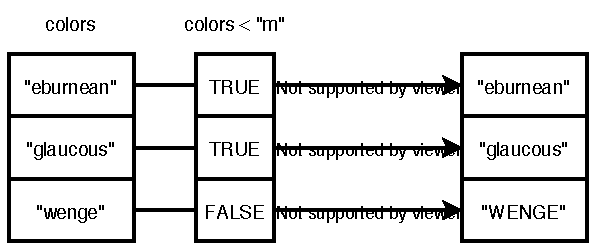
\includegraphics{figures/basics/if-else.pdf}
  \caption{Vector Conditionals}
  \label{fig:ifelse-fig}
\end{figure}

\section{The Absence of Data}

As discussed earlier,
the special value \texttt{NA} is used to represent missing data.
A different value,
\gref{g:null}{\texttt{NULL}},
represents the absence of a vector.
They are not the same thing:
\texttt{NA} means
``there is supposed to be a value here but we don't know what it is''
while \texttt{NULL} means
``we don't have a vector at all''.

\texttt{NULL} is not the same as a vector of zero length,
though testing that statement produces a rather odd result:

\begin{lstlisting}
NULL == integer(0)
\end{lstlisting}

\begin{lstlisting}
logical(0)
\end{lstlisting}

The safe way to test if something is \texttt{NULL} is to use the function \texttt{is.null}:

\begin{lstlisting}
is.null(NULL)
\end{lstlisting}

\begin{lstlisting}
[1] TRUE
\end{lstlisting}

Circling back,
the safe way to test whether a value is \texttt{NA} is \emph{not} to use direct comparison:

\begin{lstlisting}
threshold <- 1.75
threshold == NA
\end{lstlisting}

\begin{lstlisting}
[1] NA
\end{lstlisting}

The result is \texttt{NA} because if we don't know what a value is,
we can't know if it is equal to \texttt{threshold} or not.
Instead,
we should always use the function \texttt{is.na}:

\begin{lstlisting}
is.na(threshold)
\end{lstlisting}

\begin{lstlisting}
[1] FALSE
\end{lstlisting}

\begin{lstlisting}
is.na(NA)
\end{lstlisting}

\begin{lstlisting}
[1] TRUE
\end{lstlisting}

\section{Storing Mixed Types}

One of the things that newcomers to R often trip over is
the various ways in which data structures can be indexed.
All of the following may be legal:

\begin{lstlisting}
thing[i]
thing[i, j]
thing[[i]]
thing[[i, j]]
thing$name
thing$"name"
\end{lstlisting}

\noindent
but they can behave differently depending on what kind of thing \texttt{thing} is.
To understand what is possible when,
we must first take a look at lists.

A \gref{g:list}{list} in R is a vector that can contain values of many different types.
(The technical term for this is \gref{g:heterogeneous}{heterogeneous},
in contrast with a \gref{g:homogeneous}{homogeneous} data structure
that can only contain one type of value.)
We can construct a list using the \texttt{list} function:

\begin{lstlisting}
thing <- list("first", c(2, 20, 200), 3.3)
thing
\end{lstlisting}

\begin{lstlisting}
[[1]]
[1] "first"

[[2]]
[1]   2  20 200

[[3]]
[1] 3.3
\end{lstlisting}

The output tells us that the first element of \texttt{thing} is a vector of one element,
that the second is a vector of three elements,
and the third is again a vector of one element.
The major indices are shown in double square brackets \texttt{[[\ldots{}]]},
while the indices of the contained elements are shown in single square brackets \texttt{[\ldots{}]}.
(Again,
remember that \texttt{"first"} and 3.3 are actually vectors of length 1.)

\begin{quote}
\textbf{By Convention}

In keeping with R's conventions,
we will henceforth use \texttt{[[} and \texttt[ to refer to the two kinds of indexing
rather than \texttt{[[\ldots{}]]} and \texttt{[\ldots{}]}.
\end{quote}

\subsection{Single versus Double}

The output above suggests that
we can get the elements of a list using \texttt{[[}
(i.e., using double square brackets):

\begin{lstlisting}
thing[[1]]
\end{lstlisting}

\begin{lstlisting}
[1] "first"
\end{lstlisting}

\begin{lstlisting}
thing[[2]]
\end{lstlisting}

\begin{lstlisting}
[1]   2  20 200
\end{lstlisting}

\begin{lstlisting}
thing[[3]]
\end{lstlisting}

\begin{lstlisting}
[1] 3.3
\end{lstlisting}

That seems to have worked,
so let's look at the types of those three values:

\begin{lstlisting}
typeof(thing[[1]])
\end{lstlisting}

\begin{lstlisting}
[1] "character"
\end{lstlisting}

\begin{lstlisting}
typeof(thing[[2]])
\end{lstlisting}

\begin{lstlisting}
[1] "double"
\end{lstlisting}

\begin{lstlisting}
typeof(thing[[3]])
\end{lstlisting}

\begin{lstlisting}
[1] "double"
\end{lstlisting}

Again,
since everything is a vector,
those types seem sensible.
Now,
what do we get if we index single square brackets \texttt{[\ldots{}]}?

\begin{lstlisting}
thing[1]
\end{lstlisting}

\begin{lstlisting}
[[1]]
[1] "first"
\end{lstlisting}

That looks like a list, not a vector---let's check:

\begin{lstlisting}
typeof(thing[1])
\end{lstlisting}

\begin{lstlisting}
[1] "list"
\end{lstlisting}

This example shows the difference between \texttt{[[} and \texttt[:
the former peels away a layer of data structure,
returning only the sub-structure,
while the latter gives us back a structure of the same type as the thing being indexed.
Since a ``scalar'' is just a vector of length 1,
there is no difference between \texttt{[[} and \texttt[ when they are applied to vectors:

\begin{lstlisting}
v <- c("first", "second")
v[2]
\end{lstlisting}

\begin{lstlisting}
[1] "second"
\end{lstlisting}

\begin{lstlisting}
v[[2]]
\end{lstlisting}

\begin{lstlisting}
[1] "second"
\end{lstlisting}

\section{Accessing by Name}

R allows us to name the elements in vectors and lists:
if we assign \texttt{c(one = 1, two = 2, three = 3)} to \texttt{names},
then \texttt{names["two"]} is 2.
We can use this to create a lookup table:

\begin{lstlisting}
values <- c("m", "f", "nb", "f", "f", "m", "m")
lookup <- c(m = "Male", f = "Female", nb = "Non-binary")
lookup[values]
\end{lstlisting}

\begin{lstlisting}
           m            f           nb            f            f 
      "Male"     "Female" "Non-binary"     "Female"     "Female" 
           m            m 
      "Male"       "Male" 
\end{lstlisting}

If the name of the field is itself a legal variable name,
we can also use the shorthand \texttt{lookup\$m} instead of \texttt{lookup["m"]}:

\begin{lstlisting}
lookup$m
\end{lstlisting}

\begin{lstlisting}
[1] "Male"
\end{lstlisting}

We will explore this in more detail when we look at the tidyverse in Chapter~\ref{tidyverse},
since that is where access-by-name is used most often.
For now,
simply note that if the name of an element \emph{isn't} a legal variable name,
we have to put it in backward quotes to use it with \texttt{\$}:

\begin{lstlisting}
another_list <- list("first field" = "F", "second field" = "S")
another_list$`first field`
\end{lstlisting}

\begin{lstlisting}
[1] "F"
\end{lstlisting}

If you have control,
or at least the illusion thereof,
choose names such as \texttt{first\_field} that don't require back-quoting:
they are simpler both to read and to use.

\begin{quote}
\textbf{Flattening and Recursive Indexing}

If a list is just a vector of objects, why do we need the function \texttt{list}?
Why can't we create a list with \texttt{c("first", c(2, 20, 200), 30)}?
The answer is that R flattens the arguments to \texttt{c},
so \texttt{c(c(1, 2), c(3, 4))} produces \texttt{c(1, 2, 3, 4)}.
It also does automatic type conversion:
\texttt{c("first", c(2, 20, 200), 30)} produces a vector of character strings
\texttt{c("first", "2", "20", "200", "30")}.
This can be annoying even after you get used to it
(which again is true of both quantum mechanics and necromancy).

Another ``helpful, ish'' behavior is that using \texttt{[[} with a list subsets recursively:
if we assign \texttt{list(a = list(b = list(c = 1)))} to \texttt{thing},
then \texttt{thing[[c("a", "b", "c")]]} selects the value 1.
\end{quote}

\section{How can we create and index a matrix?}

Matrices are frequently used in statistics, so R provides built-in support for them.
After assigning \texttt{matrix(1:9, nrow = 3)} to a variable \texttt{a},
\texttt{a} is a 3x3 matrix containing the numbers 1 through 9:

\begin{lstlisting}
a <- matrix(1:9, nrow = 3)
a
\end{lstlisting}

\begin{lstlisting}
     [,1] [,2] [,3]
[1,]    1    4    7
[2,]    2    5    8
[3,]    3    6    9
\end{lstlisting}

Behind the scenes,
a matrix is a vector with a special property or \gref{g:attribute}{attribute} called \texttt{dim}
that stores its dimensions:

\begin{lstlisting}
dim(a)
\end{lstlisting}

\begin{lstlisting}
[1] 3 3
\end{lstlisting}

\noindent
We will look at attributes in more detail in Section~\ref{advanced-oop}.
For now,
it's enough to know that since a matrix is just a vector with pretensions of grandeur,
all the things that work for vectors also work for matrices.
For example,
\texttt{a[3, 3]} is a vector of length 1 containing the value 9
because scalars in R are actually vectors,
and we can get the same value using \texttt{a[9]}.
And if we want rows and columns,
\texttt{a[1,]} selects the first row,
giving us the vector \texttt{c(1, 4, 7)},
while \texttt{a[,1]} selects the first column
to give \texttt{c(1, 2, 3)}.

\section{Choosing and Repeating Things}

We cherish the illusion of free will so much that we embed a pretense of it in our machines
in the form of conditional statements using \texttt{if} and \texttt{else}.
(Ironically,
we then instruct those same machines to make the same decisions over and over.
It's no wonder they consider us mad{\ldots})
For example,
here is a snippet of Python that uses \texttt{for} and \texttt{if} to display
the signs of the numbers in a list:

\begin{lstlisting}
values = [-15, 0, 15]
for v in values:
    if v < 0:
        pos_neg = -1
    elif v == 0:
        pos_neg = 0
    else:
        pos_neg = 1
    print("The pos_neg of", v, "is", pos_neg)
print("The final value of v is", v)
\end{lstlisting}

\begin{lstlisting}
The pos_neg of -15 is -1
The pos_neg of 0 is 0
The pos_neg of 15 is 1
The final value of v is 15
\end{lstlisting}

Its direct translation into R is:

\begin{lstlisting}
values <- c(-15, 0, 15)
for (v in values) {
  if (v < 0) {
    pos_neg <- -1
  }
  else if (v == 0) {
    pos_neg <- 0
  }
  else {
    pos_neg <- 1
  }
  print(glue::glue("The sign of {v} is {pos_neg}"))
}
print(glue::glue("The final value of v is {v}"))
\end{lstlisting}

\begin{lstlisting}
The sign of -15 is -1
The sign of 0 is 0
The sign of 15 is 1
The final value of v is 15
\end{lstlisting}

There are a few things to note here:

\begin{enumerate}
\item
  The parentheses in the loop header are required:
  we cannot simply write \texttt{for v in values}.
\item
  The curly braces around the body of the loop
  and around the bodies of the conditional branches are optional
  if those bodies only contain a single statement as they do here.
  However,
  code is much easier to read if the braces are always present.
\item
  As in Python,
  the loop variable \texttt{v} continues to exist after the loop is over.
\item
  \texttt{glue::glue} is the function \texttt{glue} from the library of the same name.
  It formats values into strings in a variety of ways
  like the \texttt{format} method of Python strings
  or its more recent f-strings.
  (Note that R uses \texttt{::} to get functions out of packages rather than \texttt{.} like Python.)
\item
  We have called our temporary variable \texttt{pos\_neg} rather than \texttt{sign}
  so that we don't accidentally overwrite the built-in R function with that name.
  \gref{g:name-collision}{Name collisions} of this sort
  are just as easy in R as they are in Python.
\end{enumerate}

\section{Vectorizing Loops and Conditionals}

The example above is \emph{not} how we should write R:
everything in that snippet can and should be vectorized.
The simplest way to do that in this case
is to use the built-in \texttt{sign} function:

\begin{lstlisting}
print(sign(values))
print(glue::glue("The sign of {values} is {sign(values)}"))
\end{lstlisting}

\begin{lstlisting}
[1] -1  0  1
The sign of -15 is -1
The sign of 0 is 0
The sign of 15 is 1
\end{lstlisting}

\noindent
Notice here that \texttt{glue::glue} is also vectorized:
since \texttt{values} is a vector containing three numbers,
\texttt{glue::glue} produces a vector containing three strings
for \texttt{print} to display.

But what if the function we want doesn't exist
(or if we don't know what it's called)?
In that case,
the easiest approach is often to create a new vector
whose values are derived from those of the vector we had
and trust R to match up corresponding elements.
The example below creates a vector called \texttt{pos\_neg} containing our numbers' signs,
then passes that and the numbers to \texttt{glue::glue},
which runs once for each matched-up pair of sign and value:

\begin{lstlisting}
pos_neg <- dplyr::case_when(
  values <  0 ~ -1,
  values == 0 ~ 0,
  values >  0 ~ 1
)

print(glue::glue("The sign of {values} is {pos_neg}"))
\end{lstlisting}

\begin{lstlisting}
The sign of -15 is -1
The sign of 0 is 0
The sign of 15 is 1
\end{lstlisting}

The function \texttt{case\_when} is a generaliztion of \texttt{ifelse};
where the latter selects a value from one of two vectors,
\texttt{case\_when} can try any number of tests in order
and returns the value associated with the first that is true.
Each option uses the \texttt{{\textasciitilde}} operator to combine
a logical test on the left with a result on the right.
We will see other uses for \texttt{{\textasciitilde}} in subsequent chapters.

\section{Ranges of Values}

\texttt{for} in R loops over the values in a vector,
just as it does in Python.
If we want to loop over the indices instead,
we can use the function \texttt{seq\_along}:

\begin{lstlisting}
colors <- c("eburnean", "glaucous", "squamous", "wenge")
for (i in seq_along(colors)) {
  print(glue::glue("The length of color {i} is {length(colors[i])}"))
}
\end{lstlisting}

\begin{lstlisting}
The length of color 1 is 1
The length of color 2 is 1
The length of color 3 is 1
The length of color 4 is 1
\end{lstlisting}

This output makes no sense until we remember that \texttt{length} returns the length of a vector,
so that \texttt{length(colors[1])} is telling us that \texttt{colors[1]} contains one element.
If we want the number of characters in the strings,
we can use R's built-in \texttt{nchar} function or the more modern \texttt{stringr::str\_length}
as shown below:

\begin{lstlisting}
for (i in seq_along(colors)) {
  print(glue::glue("The length of color {i} is {stringr::str_length(colors[i])}"))
}
\end{lstlisting}

\begin{lstlisting}
The length of color 1 is 8
The length of color 2 is 8
The length of color 3 is 8
The length of color 4 is 5
\end{lstlisting}

As you may already have guessed,
\texttt{seq\_along} returns a vector containing the indices for a vector:

\begin{lstlisting}
seq_along(colors)
\end{lstlisting}

\begin{lstlisting}
[1] 1 2 3 4
\end{lstlisting}

Sequences of numbers are used so that
that R lets us write them using \gref{g:range-expression}{range expressions}:

\begin{lstlisting}
5:10
\end{lstlisting}

\begin{lstlisting}
[1]  5  6  7  8  9 10
\end{lstlisting}

One common use is indexing a vector:

\begin{lstlisting}
colors[2:3]
\end{lstlisting}

\begin{lstlisting}
[1] "glaucous" "squamous"
\end{lstlisting}

We can also create ranges of negative numbers
and use them to subtract elements from a vector:

\begin{lstlisting}
colors[-1:-2]
\end{lstlisting}

\begin{lstlisting}
[1] "squamous" "wenge"   
\end{lstlisting}

However, R does not allow use to specify a step size other than 1 using \texttt{start:end:step}
in the way that some languages do.
To do that,
we must use the function \texttt{seq} as shown below:

\begin{lstlisting}
seq(1, 10, 3)
\end{lstlisting}

\begin{lstlisting}
[1]  1  4  7 10
\end{lstlisting}

This example also shows that ranges in R are inclusive at both ends,
i.e.,
they run up to \emph{and including} the upper bound.
This contrasts with Python,
where an expression like \texttt{vec[0:4]} gets elements up to but \emph{not} including the fourth.
As is traditional among programming language advocates,
the users of each language claim that their preferred behavior is more natural
and then cite some supportive anecdote as if it were proof.

\begin{quote}
\textbf{Repeating Things}

The function \texttt{rep} repeats things,
so \texttt{rep("a", 3)} is \texttt{c("a", "a", "a")}.
If the second argument is a vector of the same length as the first,
it specifies how many times each item in the first vector is to be repeated:
\texttt{rep(c("a", "b"), c(2, 3))} is \texttt{c("a", "a", "b", "b", "b")}.
\end{quote}

\section{Vectors in Conditional Tests}

We cannot use a vector with multiple values as a condition in an \texttt{if} statement
because R cannot know which of the values it should base its decision on.
For example,
if a vector contains both 0 (which counts as false) and 1 (which counts as true),
R would either have to follow some arbitrary rule about which to pay attention to
or enter some strange quantum state in which it has both taken and not taken a decision.
Instead,
it simply tells us ``no'' as shown below:

\begin{lstlisting}
numbers <- c(0, 1)
if (numbers) {
  print("This should not work.")
}
\end{lstlisting}

\begin{lstlisting}
Warning in if (numbers) {: the condition has length > 1 and only the first
element will be used
\end{lstlisting}

To get a single unambiguous value for R to work on,
we must collapse the vector into a single logical value.
The function \texttt{all} returns true if all of its inputs are true;
it corresponds to a logical ``and'' of all its inputs:

\begin{lstlisting}
numbers <- c(0, 1)
if (all(numbers >= 0)) {
  print("This, on the other hand, should work.")
}
\end{lstlisting}

\begin{lstlisting}
[1] "This, on the other hand, should work."
\end{lstlisting}

We can use a corresponding function \texttt{any} to check if at least one value is \texttt{TRUE},
which corresponds to a logical ``or'' across the whole input.

\section{Creating and Calling Functions}

As we have already seen,
we call functions in R just as we do in Python:

\begin{lstlisting}
max(1, 3, 5) + min(1, 3, 5)
\end{lstlisting}

\begin{lstlisting}
[1] 6
\end{lstlisting}

We define a new function using the \texttt{function} keyword.
This creates the function,
but does \emph{not} give it a name the way \texttt{def} does in Python.
To do that,
we must assign the newly-created function to a variable:

\begin{lstlisting}
swap <- function(pair) {
  c(pair[2], pair[1])
}
swap(c("left", "right"))
\end{lstlisting}

\begin{lstlisting}
[1] "right" "left" 
\end{lstlisting}

As the example above shows,
the result of a function is the value of the last expression evaluated within it.
A function can return a value earlier using the \texttt{return} function;
we can use \texttt{return} for the final value as well,
but most R programmers do not.
For example,
a novice R programmer might write this:

\begin{lstlisting}
swap <- function(pair) {
  if (length(pair) != 2) {
    return(NULL) # This is very bad practice.
  }
  c(pair[2], pair[1])
}
swap(c("one"))
\end{lstlisting}

\begin{lstlisting}
NULL
\end{lstlisting}

\begin{lstlisting}
swap(c("left", "right"))
\end{lstlisting}

\begin{lstlisting}
[1] "right" "left" 
\end{lstlisting}

Returning \texttt{NULL} when our function's inputs are invalid as we have done above is foolhardy,
as doing so means that \texttt{swap} can fail without telling us that it has done so.
For example,
if we call \texttt{swap} on a vector with more than two values
it \emph{seems} to work:

\begin{lstlisting}
values <- 5:10
result <- swap(values)
\end{lstlisting}

\noindent
but look what happens if we try to get one of the ``swapped'' values:

\begin{lstlisting}
result[1]
\end{lstlisting}

\begin{lstlisting}
NULL
\end{lstlisting}

\noindent
R produces this strange result because \texttt{NULL}
can be indexed like any other vector:

\begin{lstlisting}
NULL[1]
\end{lstlisting}

\begin{lstlisting}
NULL
\end{lstlisting}

We will look at what we \emph{should} do when given invalid inputs in Chapter~\ref{testerror}.

\section{Functions with Variable Arguments}

If the number of arguments given to a function is not the number that function expects,
R complains:

\begin{lstlisting}
swap("one", "two", "three")
\end{lstlisting}

\begin{lstlisting}
Error in swap("one", "two", "three"): unused arguments ("two", "three")
\end{lstlisting}

\noindent
(Note that we are passing three separate values here,
not a single vector containing three values.)
If we want a function to handle a \gref{g:variable-arguments}{varying number of arguments},
we represent the ``extra'' arguments with an ellipsis \texttt{...} (three dots),
which serves the same purpose as Python's \texttt{*args}.
In many cases,
we will simply pass these extra arguments to another function like \texttt{paste},
which creates a string by combining its arguments with the specified separator
as shown below:

\begin{lstlisting}
print_with_title <- function(title, ...) {
  print(glue::glue("=={title}=="), paste(..., sep = "\n"))
}

print_with_title("to-do", "Monday", "Tuesday", "Wednesday")
\end{lstlisting}

\begin{lstlisting}
==to-do==
Monday
Tuesday
Wednesday
\end{lstlisting}

R uses a special data structure to represent the extra arguments in \texttt{...}.
If we want to access those arguments one by one,
we must convert \texttt{...} to a list.
The function below does this so that it can loop over those values:

\begin{lstlisting}
add <- function(...) {
  result <- 0
  for (value in list(...)) {
    result <- result + value
  }
  result
}
add(1, 3, 5, 7)
\end{lstlisting}

\begin{lstlisting}
[1] 16
\end{lstlisting}

\section{Default Values for Arguments}

Like Python and most other modern programming languages,
R lets us define default values for arguments
and then pass values to functions by name.
The \texttt{example} function below shows
how this works when named and unnamed values are both provided:

\begin{lstlisting}
example <- function(first, second = "second", third = "third") {
  print(glue::glue("first='{first}' second='{second}' third='{third}'"))
}

example("with just first")
\end{lstlisting}

\begin{lstlisting}
first='with just first' second='second' third='third'
\end{lstlisting}

\begin{lstlisting}
example("with first and second by position", "positional")
\end{lstlisting}

\begin{lstlisting}
first='with first and second by position' second='positional' third='third'
\end{lstlisting}

\begin{lstlisting}
example("with first and third by name", third = "by name")
\end{lstlisting}

\begin{lstlisting}
first='with first and third by name' second='second' third='by name'
\end{lstlisting}

\begin{quote}
\textbf{Two Hours Later{\ldots}}

R has a peculiar tendency to ignore things that \emph{aren't} functions
when asked to call things that are.
This is why the call to \texttt{orange()} in the code below
produces 110 rather than an error:
\texttt{purple(purple)} is interpreted as
``pass the value 10 into the globally-defined function \texttt{purple}''
rather than ``try to call a function \texttt{10(10)}''.

\begin{lstlisting}
purple <- function(x) x + 100
orange <- function() {
  purple <- 10
  purple(purple)
}
orange()
\end{lstlisting}

\begin{lstlisting}
[1] 110
\end{lstlisting}

\noindent
This ``helpful'' behavior may surprise programmers coming from other languages{\ldots}

\end{quote}

\section{Running Quietly}

If the value returned by a function isn't assigned to something,
R displays it.
Since this usually isn't how we want a library function to behave,
we can use the function \texttt{invisible} to mark a value as ``not to be printed''
(though it can still be assigned as usual).
For example,
we can convert this function:

\begin{lstlisting}
something <- function(value) {
  10 * value
}
something(2)
\end{lstlisting}

\begin{lstlisting}
[1] 20
\end{lstlisting}

\noindent
to this:

\begin{lstlisting}
something <- function(value) {
  invisible(10 * value)
}
something(2)
\end{lstlisting}

The calculation is still being done,
but the output is not printed unless the user prints it.

\section{Assigning to Global Variables}

The assignment operator \texttt{\textless{}\textless{}-} means
``assign to a variable outside the current scope''.
Having a special form of assignment for this may seem odd
given that other languages don't have it,
but it tells readers what effect the assignment is going to have
right where the assignment takes place.
The example below shows its effect:

\begin{lstlisting}
var <- "original value"

demonstrate <- function() {
  var <<- "new value"
}

demonstrate()
var
\end{lstlisting}

\begin{lstlisting}
[1] "new value"
\end{lstlisting}

Even with this extra signalling,
global variables should only be modified rarely and carefully:
\emph{nobody} thinks that global state is a good idea any longer.

\section{Key Points}

\begin{itemize}
\item
  Use \texttt{print(expression)} to print the value of a single expression.
\item
  Variable names may include letters, digits, \texttt{.}, and \texttt{\_}, but \texttt{.} should be avoided, as it sometimes has special meaning.
\item
  R's atomic data types include logical, integer, double (also called numeric), and character.
\item
  R stores collections in homogeneous vectors of atomic types, or in heterogeneous lists.
\item
  `Scalars' in R are actually vectors of length 1.
\item
  Vectors and lists are created using the function \texttt{c(...)}.
\item
  Vector indices from 1 to length(vector) select single elements.
\item
  Negative indices to vectors deselect elements from the result.
\item
  The index 0 on its own selects no elements, creating a vector or list of length 0.
\item
  The expression \texttt{low:high} creates the vector of integers from \texttt{low} to \texttt{high} inclusive.
\item
  Subscripting a vector with a vector of numbers selects the elements at those locations (possibly with repeats).
\item
  Subscripting a vector with a vector of logicals selects elements where the indexing vector is \texttt{TRUE}.
\item
  Values from short vectors (such as `scalars') are repeated to match the lengths of longer vectors.
\item
  The special value \texttt{NA} represents missing values, and (almost all) operations involving \texttt{NA} produce \texttt{NA}.
\item
  The special values \texttt{NULL} represents a nonexistent vector, which is not the same as a vector of length 0.
\item
  A list is a heterogeneous vector capable of storing values of any type (including other lists).
\item
  Indexing with \texttt{[} returns a structure of the same type as the structure being indexed (e.g., returns a list when applied to a list).
\item
  Indexing with \texttt{[[} strips away one level of structure (i.e., returns the indicated element without any wrapping).
\item
  Use \texttt{list('name' = value, ...)} to name the elements of a list.
\item
  Use either \texttt{L['name']} or \texttt{L\$name} to access elements by name.
\item
  Use back-quotes around the name with \texttt{\$} notation if the name is not a legal R variable name.
\item
  Use \texttt{matrix(values, nrow = N)} to create a matrix with \texttt{N} rows containing the given values.
\item
  Use \texttt{m[i, j]} to get the value at the i'th row and j'th column of a matrix.
\item
  Use \texttt{m[i,]} to get a vector containing the values in the i'th row of a matrix.
\item
  Use \texttt{m[,j]} to get a vector containing the values in the j'th column of a matrix.
\item
  Use \texttt{for (loop\_variable in collection)\{ ...body... \}} to create a loop.
\item
  Use \texttt{if (expression) \{ ...body... \} else if (expression) \{ ...body... \} else \{ ...body... \}} to create conditionals.
\item
  Expression conditions must have length 1; use \texttt{any(...)} and \texttt{all(...)} to collapse logical vectors to single values.
\item
  Use \texttt{function(...arguments...) \{ ...body... \}} to create a function.
\item
  Use variable \textless{}- function(\ldots{}arguments\ldots{}) \{ \ldots{}body\ldots{} \}` to create a function and give it a name.
\item
  The body of a function can be a single expression or a block in curly braces.
\item
  The last expression evaluated in a function is returned as its result.
\item
  Use \texttt{return(expression)} to return a result early from a function.
\end{itemize}

\section{Exercises}

\begin{enumerate}

\item
Translate the following Python program into R.

\begin{lstlisting}
def isOdd(num):
    return (num % 2) == 0

values = range(3:10)
count = 0
for v in values:
    if isOdd(v):
        count += 1
print(count, 'are odd')
\end{lstlisting}

\item
The following program:

\begin{lstlisting}
values <- list(0, c(), FALSE, NA)
for (v in values) {
  print(glue::glue("The type of {v} is {typeof(v)}")
}
\end{lstlisting}

\noindent
prints:

\begin{lstlisting}
The type of 0 is double
  
The type of FALSE is logical
The type of NA is logical
\end{lstlisting}

Explain each of the four lines of output (including the blank line).

\item
We would like to translate this nested list from Python to R:

\begin{lstlisting}
nested = ['west', ['southwest', 'southeast'], 'east']
\end{lstlisting}

\noindent
Our first attempt is:

\begin{lstlisting}
nested <- c('west', c('southwest', 'southeast'), 'east')
\end{lstlisting}

However, this produces a flat list with four elements:

\begin{lstlisting}
print(length(nested))
\end{lstlisting}

\begin{lstlisting}
[1] 4
\end{lstlisting}

\begin{enumerate}

\item
  Modify the R so that it does the same thing as the Python,
  i.e.,
  produces a list of three elements,
  the second of which is a list of two elements.

\item
  In Python,
  the expression \texttt{nested[0][0]} will get the first character of the first element of the list.
  What does the equivalent expression \texttt{nested[1][1]} get in R?
  What expression will get the first element's first character?
\end{enumerate}

\item
R allows us to store name-value pairs in a \gref{g:named-list}{named list},
which works much like a dictionary in Python:

\begin{lstlisting}
purple <- list(red=192, green=128, blue=255)
purple$red
\end{lstlisting}

\begin{lstlisting}
[1] 192
\end{lstlisting}

Write a function called \texttt{conflict}
that takes two named lists called \texttt{left} and \texttt{right} as inputs
and produces a vector containing the keys that are in both inputs but have different values:

\begin{lstlisting}
purple <- list(red=192, green=128, blue=255)
brown <- list(red=192, green=128, blue=0)
conflict(purple, brown)
\end{lstlisting}

\begin{lstlisting}
[1] "blue"
\end{lstlisting}

Don't hesitate to search online for more information.

\item
What does \texttt{seq\_along(4)} return, and why?

\end{enumerate}
